\chapter{Correlation based penalty function}

In this chapter, we propose a novel regularization factor to penalize the use of features highly correlated with a protected attribute by a machine learning model, aiming to avoid the redlining effect~\citep{Pedreschi2008}. The proposed penalization factor is applied directly to the input weights of a Multi-Layer Perceptron, using a strategy that proportionately penalizes features use based on their correlation with the sensitive feature.

\section{Preliminaries}

The phenomena known as redlining effect~\citep{Pedreschi2008} consists in the unintended use of proxy variables to the sensitive feature by the model, which can lead model to produce indirect discrimination in their outcomes.  Thus, the insight here is to penalize the use of those proxy features by the model proportionally according its correlation with sensitive feature in order to avoid redlining effed. The proposed regularization approach uses the recently described Chatterjee's xi correlation coefficient~\cite{chatterjee2020new}, which robustly asses whether a random variable can be described as a function of another one, as a measure of the potential of given feature to be used by the model as a proxy to the sensitive feature. 

Before discussing this approach, we start defining some common correlation coefficients and providing a proper comparison within Chatterjee's correlation. Also, we present some related approaches, specially those ones that, like ours, use regularization and penalty factors to avoid indirect discrimination.

The Pearson correlation coefficient, denoted by $\rho$ and defined in Definition~\ref{def:pearson}, is a measure of the linear relationship between two random variables. The Pearson correlation coefficient ranges from $-1$ to $1$, where $1$ indicates a perfect positive linear relationship, $-1$ indicates a perfect negative linear relationship, and $0$ indicates no linear relationship.

\begin{definition}[Pearson correlation coefficient]\label{def:pearson}
Let  $X$ and $Y$\ random variables. The Pearson correlation coefficient $\rho$ between $X$ and $Y$ can be defined as  
\begin{equation}
\rho = \frac{\mathrm{Cov}(X, Y)}{\sigma_X \sigma_Y},
\end{equation}
where $\mathrm{Cov}(X, Y)$ is the covariance between $X$ and $Y$, while $\sigma_X$ and $\sigma_Y$ the standard deviations of $X$ and $Y$, respectively. 
\end{definition}

Spearman's rank correlation coefficient, denoted by $\rho_s$ and defined in Definition~\ref{def:spearman}, measures the strength and direction of the monotonic relationship between two ranked (ordered) variables.  As like Pearson correlation coefficient, Spearman's rank correlation coefficient ranges from $-1$ to $1$, where $1$ indicates a perfect positive relationship, $-1$ indicates a perfect negative relationship, and $0$ indicates no relationship.
 
\begin{definition}[Spearman's correlation coefficient]\label{def:spearman}
Let $X$ and $Y$\ random variables, $n$ the sample size and $X_i, \, Y_i$ the $i$-th observations to $i = 1 \ldots n$. Let $R_{X_i}, \, R_{Y_i}$ the rank of observations $X_i, \, Y_i$, i.e. the position of $X_i, \, Y_i$ by ordering the samples, respectively. The Spearman's rank correlation coefficient  $\rho_s$ between $X$ and $Y$ can be defined to non-repeated observation values as 
\begin{equation}\label{eq:spearman}
\rho_s = 1 - \frac{6 \sum\limits_{i=1}^{n}d_i^2}{n(n^2 - 1)},
\end{equation}
where $d_i = R_{X_i} - R_{Y_i}$.
\end{definition}

Kendall's rank correlation coefficient, denoted by $\tau$ and defined in Definition~\ref{def:kendall},  indicates the strength and direction of association between two variables. It is based on the relative ordering of pairs of observations rather than their actual values. Here we interpret the correlation values as like in Spearman's and Pearson's correlation coefficients, ranging from $-1$ to $1$, where $1$ indicates a perfect positive relationship, $-1$ a perfect negative relationship, and $0$  no linear relationship.

\begin{definition}[Kendall's correlation coefficient]\label{def:kendall}
Let two variables $X$ and $Y$ sampled with $n$ pairs of observations $(X_i, Y_i)$ for $i = 1, 2, \ldots, n$. A pair of observations $(X_i, Y_i)$ and $(X_j, Y_j)$ is \textbf{concordant} if the ranks (order) of both elements agree, i.e., to $i < j$ either $X_i > X_j$ and $Y_i > Y_j)$ or $X_i < X_j$ and $Y_i < Y_j$. Otherwise their are considered \textbf{discordant}, i.e., either $X_i > X_j$ and $Y_i < Y_j$ or $X_i < X_j$ and $Y_i > Y_j$. The Kendall's rank correlation coefficient $\tau$ between $X$ and $Y$ can be defined as 
\begin{equation}\label{eq:kendall}
\tau = \frac{2(N_c - N_d)}{n(n-1)},
\end{equation}
where $N_c$ is the number of concordant observation and $N_d$ the number of discordant observations.
\end{definition}

Chatterjee's correlation coefficient, denoted by $\xi$, is designed to measure the degree of dependence between two variables without assuming any specific type of relationship. Given a dataset $(X, Y)$ with $n$ pairs, the coefficient is defined as
\begin{equation}
\xi_n(X,Y) = 1 - \frac{3 \sum_{i=1}^{n-1} |r_{i+1} - r_i|}{n^2 - 1},
\end{equation}
where $r_i$ is the rank of $Y_i$ in the ordered sequence of $Y$ values corresponding to the sorted $X$ values. This coefficient ranges from 0 to 1, where 0 indicates independence and 1 indicates a perfect functional relationship. For the general case with ties, a more complex formula involving additional terms to handle the ties is used.

% TODO (P1) (Normalization). ξ ∈ [0,1], for all distributions of (X,Y ). (P2) (Perfect dependence). ξ = 1 (reaches its maximum) if and only if there is a measurable function f : R → R, such that Y = f(X) almost surely. (P3) (D-Consistency). ξ = 0 (reaches its minimum) if and only if X and Y are independent.

\begin{table}[ht]
\centering
\caption{Anscombe's quartet}
\label{tab:valores}
\begin{tabular}{rr|rr|rr|rr}
\toprule
\multicolumn{2}{c|}{I} & \multicolumn{2}{c|}{II} & \multicolumn{2}{c|}{III} & \multicolumn{2}{c}{IV} \\

\multicolumn{1}{c}{$x$} & \multicolumn{1}{c|}{$y$} & \multicolumn{1}{c}{$x$} & \multicolumn{1}{c|}{$y$} & \multicolumn{1}{c}{$x$} & \multicolumn{1}{c|}{$y$} & \multicolumn{1}{c}{$x$} & \multicolumn{1}{c}{$y$} \\
\midrule
10.0 & 8.04 & 10.0 & 9.14 & 10.0 & 7.46 & 8.0 & 6.58 \\
8.0 & 6.95 & 8.0 & 8.14 & 8.0 & 6.77 & 8.0 & 5.76 \\
13.0 & 7.58 & 13.0 & 8.74 & 13.0 & 12.74 & 8.0 & 7.71 \\
9.0 & 8.81 & 9.0 & 8.77 & 9.0 & 7.11 & 8.0 & 8.84 \\
11.0 & 8.33 & 11.0 & 9.26 & 11.0 & 7.81 & 8.0 & 8.47 \\
14.0 & 9.96 & 14.0 & 8.10 & 14.0 & 8.84 & 8.0 & 7.04 \\
6.0 & 7.24 & 6.0 & 6.13 & 6.0 & 6.08 & 8.0 & 5.25 \\
4.0 & 4.26 & 4.0 & 3.10 & 4.0 & 5.39 & 19.0 & 12.50 \\
12.0 & 10.84 & 12.0 & 9.13 & 12.0 & 8.15 & 8.0 & 5.56 \\
7.0 & 4.82 & 7.0 & 7.26 & 7.0 & 6.42 & 8.0 & 7.91 \\
5.0 & 5.68 & 5.0 & 4.74 & 5.0 & 5.73 & 8.0 & 6.89 \\
\bottomrule
\end{tabular}
\end{table}

\begin{figure}[!ht]
\centering
\caption{Multiple correlation coefficients on Anscombe's quartet.}
    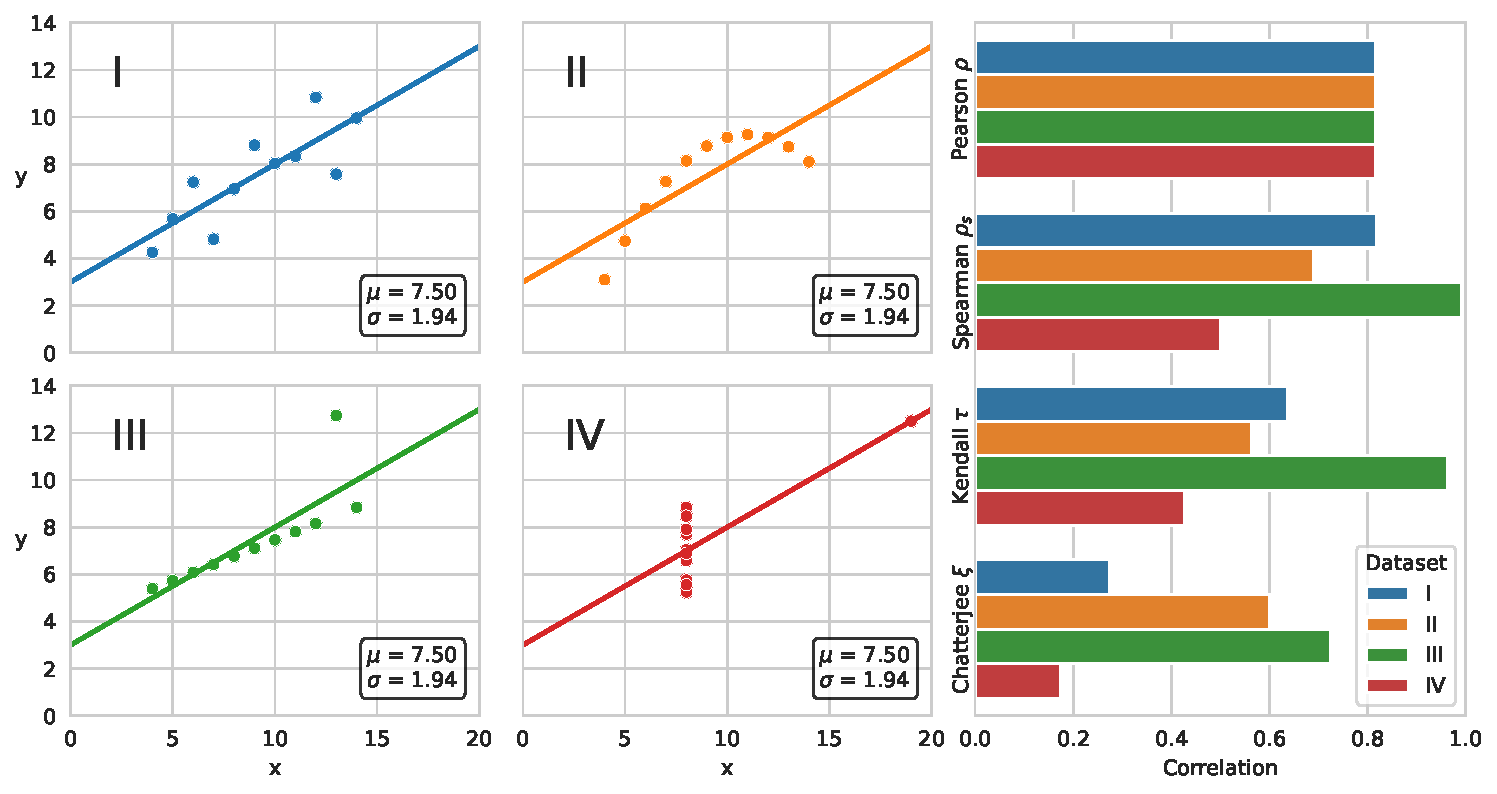
\includegraphics[width=1\linewidth]{images/anscombe_quartet.pdf}
\end{figure}



L2 regularization, also known as weight decay, is a common technique used to prevent overfitting in machine learning models, including Multi-Layer Perceptrons (MLPs). In the context of an MLP, L2 regularization adds a penalty term to the loss function that is proportional to the sum of the squares of the model parameters (weights). This encourages the model to keep the weights small, which can help improve generalization.

Let $\mathbf{W}^{(l)}$ represent the weight matrix for the $l$-th layer of the MLP, and let $\mathbf{b}^{(l)}$ denote the corresponding bias vector. The primary loss function of the network, $L_0$, could be any suitable loss function such as the mean squared error for regression or the cross-entropy loss for classification. The L2 regularization term for a single layer is given by
\begin{equation}
R(\mathbf{W}^{(l)}) = \frac{1}{2} \sum_{i=1}^{d_l} \sum_{j=1}^{h_l} \left( W^{(l)}_{ij} \right)^2,
\end{equation}
where $d_l$ and $h_l$ are the dimensions of the weight matrix $\mathbf{W}^{(l)}$, and $W^{(l)}_{ij}$ is the weight connecting the $i$-th input neuron to the $j$-th neuron in the $l$-th layer. Thus, the total regularization term for the entire network, considering all layers, is
\begin{equation}
R(\mathbf{W}) = \frac{1}{2} \sum_{l=1}^{L} \sum_{i=1}^{d_l} \sum_{j=1}^{h_l} \left( W^{(l)}_{ij} \right)^2,
\end{equation}
where $L$ is the total number of layers in the network. Furthermore, the total loss function $L$ for the MLP, incorporating the L2 regularization term, is defined as
\begin{equation}
L = L_0 + \lambda \; R(\mathbf{W}),
\end{equation}
where $\lambda$ is a scalar hyperparameter that controls the overall strength of the regularization.

By adding this regularization term, the optimization process aims to minimize the primary loss $L_0$ along with keeping the weights small, thereby helping to reduce the model complexity and prevent overfitting. The gradient descent updates for the weights will be adjusted to account for the regularization term, effectively shrinking the weights during the training process.

\section{Chatterjee Redlining Penalty}

The Chatterjee Redlining Penalty (CRP) is a regularization term that penalizes the weights of features highly correlated with the sensitive attribute, as measured by Chatterjee's Xi Rank Correlation Coefficient. By incorporating this penalty into the loss function of the neural network, the model is encouraged to reduce its reliance on sensitive attributes, thus promoting fairer predictions.

As referred before, the Chatterjee Xi Correlation Coefficient distinguish from many other by providing a measure of how much one random variable can be expressed as a function of another, with a range from $0$ to $1$. This characteristics is relevant to the proposed use, to capture redlining effect, as of this phenomena happens exactly when the sensitive feature can be inferred by another one, producing the same harmful effects whether the correlation is positive or negative. Naturally it would be possible to use the absolute value of a correlation coefficient such as Pearson or Spearman, but this strategy could lead to some kind of information loss. Another relevant characteristics of this correlation coefficient it is the ability to capture sophisticated nonlinearities and the effects of noise on variable's distribution, conditions frequently present in proxy feature relationships. 

Thus, let $X \in \mathbb{R}^{n \times d}$ be a dataset where $n$ represents the number of instances and $d$ represents the number of features. Let $X_i \in \mathbb{R}^n$ denote the $i$-th feature of the dataset, and let $A = X_i \in \mathbb{R}^n$ be a sensitive (protected) feature for some $i$. In this neural network, $\mathbf{W}^{(1)} \in \mathbb{R}^{d \times h}$ is the weight matrix for the first hidden layer, with $h$ being the number of neurons in this layer. Additionally, $\lambda$ is a scalar that controls the overall strength of the regularization.

Thus, the proposed regularization term $R(\mathbf{W}^{(1)})$ applied to the weight matrix $\mathbf{W}^{(1)}$ of the first hidden layer is defined as 
\begin{equation}\label{eq:xi_reg}
R(\mathbf{W}^{(1)}) = \sum_{i=1}^d \xi_n(X_i,\,A) \sum_{j=1}^h (W^{(1)}_{ij})^2,
\end{equation}
where $W^{(1)}_{ij}$ are the weights connecting the $i$-th input feature to the $j$-th neuron in the first hidden layer. Here, the Chatterjee's Xi Correlation Coefficient $\xi_n(X_i,\,A)$ between the $i$-th input feature $X_i$ and the sensitive feature $A$ acts as the regularization strength for the $i$-th input feature. The greater $i$-th input feature dependence on sensitive feature the greater the penalization factor enforcing lower values to those weights.

Thus, the total loss function $L$ to a MLP, incorporating the sensitive-feature-specific $L_2$ regularization, is defined as
\begin{equation}\label{eq:total_regularized_loss}
L = L_0 + \lambda \; R(\mathbf{W}^{(1)}),
\end{equation}
where $L_0$ is the primary loss function of the network. This formulation ensures that the model's learning process penalizes weights with high values associated with features highly correlated to the sensitive attribute, thereby reducing the potential for biased decisions influenced by redlining effect.

This formulation differs from similar approaches to regularization in order to achieve fairness in machine learning by two fundamental points.  The first one is that here the regularization acts as a focused penalty factor through the use of the correlation of each feature to the sensitive one, reducing it's effect on less correlated features and boosting on the highly correlated ones. The second point is that this proposed penalty does not acts as a common regularizer by imposing small values on every model's parameter. Rather, it penalizes the use of each feature according it's correlation to the sensitive one by exclusively acting on the input layer weights, that is, the usage level of each feature by hidden units.

With the combination of characteristics tailored by this formulation and the chosen correlation coefficient we do expects effectively avoiding the use of indirect sensitive feature predictors within the model, thus mitigating redlining effect.

\section{Experimental setup}

In this section, we detail the experimental setup employed to benchmark the proposed regularization within both Standard MLP with Cross Entropy Loss and a MLP using Fair Transition Loss. Both MLP model uses two hidden layers with $100$ hidden units each, $ReLU$ activation function, batch size of $64$, $50$ epochs early stopped at $3$ epochs without improvement~\citep{Li2020} and softmax in output, trained with ADAM optimizer~\citep{KingmaB14} and learning rate at $3\mathrm{e}{-4}$. 

The experimental methodology follows same principles of the one used on Fair Transition Loss Evaluation. There are two phases: hyperparameter tuning and testing. In the hyperparameter tuning phase we perform a Bandit-Based pruning approach using HyperBand~\citep{Li2018} with Tree-structured Parzen Estimator Sampler (TPE)~\citep{bergstra2011} over $100$ trials. At each trial a fitness function is evaluated by performing a complete training and validation, where both model performance and fairness metrics are assessed. The fitness function is computed based on the objective defined in Equation~\ref{eq:obj_fn}. 

Once the best hyperparameters are selected, we proceed to the testing phase, where a new training is conducted using those optimal hyperparameters. After this training, we evaluate the model's performance on a separate test set that was not used during the hyperparameter tuning phase, which are reported. This complete tuning-training-testing described is repeated $15$ times with dataset re-sampling then we proceed to comparison. Here the re-sampling consists in shuffling the whole dataset before splitting, which is better described further in this section.

As the objective defined in Equation~\ref{eq:obj_fn} can be achieved with different performance and fairness metrics, we compare the proposed regularization schema within Standard MLP and MLP with FTL in different optimization scenarios, considering as performance metrics Accuracy (Acc.) and Mathews Correlation Coefficient (MCC), while the fairness metrics considered are Statistical Parity (Stat. Parity), Equal Opportunity (Eq. Opp.) and Equalized Odds (Eq. Odds). Those pursued metrics lead us to the following optimization scenarios: MCC and Statistical Parity; MCC and Equal Opportunity; MCC and Equalized Odds; Accuracy and Statistical Parity; Accuracy and Equal Opportunity; Accuracy and Equalized Odds.

\begin{table}[ht]
\centering
\caption{Hyperparameters search ranges or options of each method.}\label{tab:hyperparameters_crp}
{\footnotesize
\begin{tabular}{lll}
\toprule
Method & Parameter & Range/options \\ \midrule
 Standard MLP without regularization (baseline) & dropout & $[0.0,\,0.2]$  \vspace{1ex} \\
 Standard MLP with CRP & dropout & $[0.0,\,0.2]$  \vspace{1ex} \\
 & $\lambda$ & $\{1e^{-2}, 1^{e-3}, 1^{e-4}\}$ \\
 Fair Transition Loss without regularization & $d_0,p_0,d_1,p_1$ & $[0.0,\,1.0]$ \\
 &  dropout & $[0.0,\,0.2]$ \\
 Fair Transition Loss with CRP & $d_0,p_0,d_1,p_1$ & $[0.0,\,1.0]$ \\
 &  dropout & $[0.0,\,0.2]$ \\
 & $\lambda$ & $\{1e^{-2}, 1^{e-3}, 1^{e-4}\}$ \\
\bottomrule
\end{tabular}
}
\end{table}

Table~\ref{tab:hyperparameters_crp} presents the methods hyperparameters along with their corresponding search ranges or options. While each method may possess a varying number of hyperparameters and range sizes, all are optimized under the same conditions and number of configurations to guarantee a balanced comparison.

To properly compare this set of $15$ results of each method, we conduct an Almost Stochastic Order (ASO) test \citep{dror2019deep}, a significance test suitable for comparing complex machine learning models with various hyperparameters. The ASO test involves evaluating a set of metrics through multiple samplings of a Collection of Statistics (in this case assessed in test phase using random resampling) to compare one method against another. The $ASO(A, B)$ function yields a value in the range $[0, 1]$, given two methods $A$ and $B$. If $ASO(A, B)$ is lesser than $0.5$, we can reject the null hypothesis and conclude that method $A$ outperforms method $B$ in the given task. That is, method $A$ produces stochastically larger values than method $B$ for a given metric. The lower the $ASO(A, B)$ value, the stronger the evidence that $A$ is superior to $B$ in that particular task, which can be interpreted as a confidence interval. Therefore, we perform pairwise comparisons between all methods for each optimization scenario outlined previously and for each dataset.

Our experiments uses common datasets used in Fair Classification problems, namely \textit{Adult Income}~\citep{misc_adult_2}, \textit{German Credit}~\citep{misc_statlog_(german_credit_data)_144}, \textit{Bank Marketing}~\citep{misc_bank_marketing_222}, and \textit{COMPAS Recidivism}~\citep{misc_compas}. We use the dataset readers available in the AI Fairness 360 toolkit~\citep{aif360-oct-2018} with its standard configurations. Instances with missing data are removed. To a proper description of those datasets please check Section~\ref{sec:experimental}


For all datasets, the data preparation process is the same, one-hot encoding for categorical features and standardize the numerical features. We perform a random split, with $80\%$ allocated for the hyperparameter tuning phase and the remaining $20\%$ reserved for evaluating metrics in the test phase. Within the hyperparameter tuning phase, this corresponding fraction of data is further randomly split, with $80\%$ assigned to training and $20\%$ to validation. The validation set allows us to assess metrics and compute the fitness function for each hyperparameter configuration. In datasets where there is originally some kind of split (e.g., train set and test set in separate files), all available data is merged and then shuffled to produce new splits at each run.

\section{Results and discussion}


\begin{table}[ht]
\centering
\caption{Almost Stochastic Order test comparing the use of Chatterjee Redlining Penalty on Standard MLP and MLP with Fair Transition Loss fitness. Values under $0.5$ (in bold) mean that the model with CRP outperforms the same model without regularization on each optimization scenario.} \label{tab:aso_compare_crp}
{\footnotesize
\begin{tabular}{lrrrr|rrrr}
\toprule
\multirow{2}{*}{Fitness Rule} & \multicolumn{4}{c}{MLP} & \multicolumn{4}{c}{FTL} \\
& Adult & Bank & Compas & German & Adult & Bank & Compas & German \\
\midrule
MCC - S. Parity & 0.79 & 0.99 & \textbf{0.03} & 1.00 & \textbf{0.34} & 1.00 & 1.00 & \textbf{0.31} \\
MCC - Eq. Opp. & \textbf{0.26} & 1.00 & \textbf{0.01} & 1.00 & \textbf{0.35} & 1.00 & \textbf{0.19} & 1.00 \\
MCC - Eq. Odds & \textbf{0.08} & 1.00 & \textbf{0.20} & 1.00 & \textbf{0.30} & 1.00 & 0.56 & 1.00 \\
Acc. - S. Parity & 0.75 & 1.00 & \textbf{0.39} & 0.87 & \textbf{0.44} & 1.00 & \textbf{0.02} & 1.00 \\
Acc. - Eq. Opp. & 1.00 & \textbf{0.18} & \textbf{0.07} & \textbf{0.24} & 0.58 & 0.67 & 1.00 & 1.00 \\
Acc. - Eq. Odds & \textbf{0.33} & 1.00 & \textbf{0.01} & 0.62 & \textbf{0.40} & 1.00 & \textbf{0.20} & 1.00 \\
\bottomrule
\end{tabular}
}
\end{table}


\begin{figure}[!ht]
\centering
\caption{Fitness values of CRP optimizing MCC and multiple fairness metrics.}
\begin{subfigure}{.32\linewidth}
    \caption{Statistical Parity}
    \label{fig:boxplot_mcc_parity_crp}
    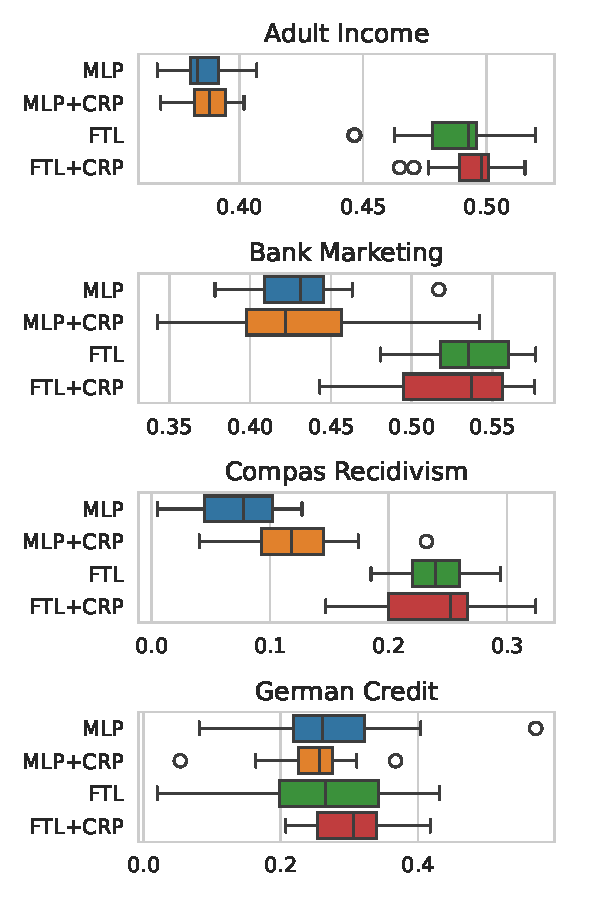
\includegraphics[width=1\linewidth]{images/boxplot_mcc_parity_crp.pdf}
\end{subfigure}
\begin{subfigure}{.32\linewidth}
    \caption{Equal Opportunity}
    \label{fig:boxplot_mcc_opp_crp}
    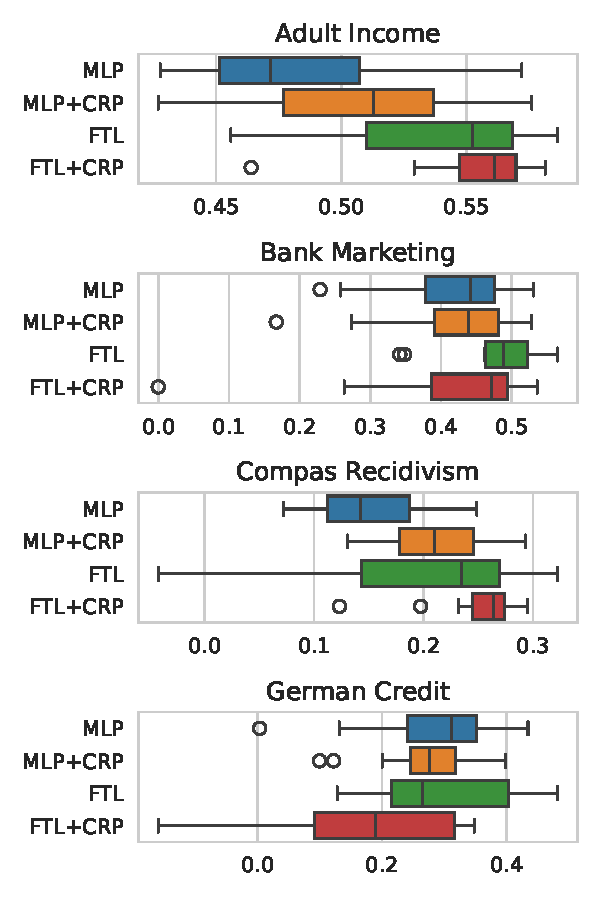
\includegraphics[width=1\linewidth]{images/boxplot_mcc_opportunity_crp.pdf}
\end{subfigure}
\begin{subfigure}{.32\linewidth}
    \caption{Equalized Odds}
    \label{fig:boxplot_mcc_odds_crp}
    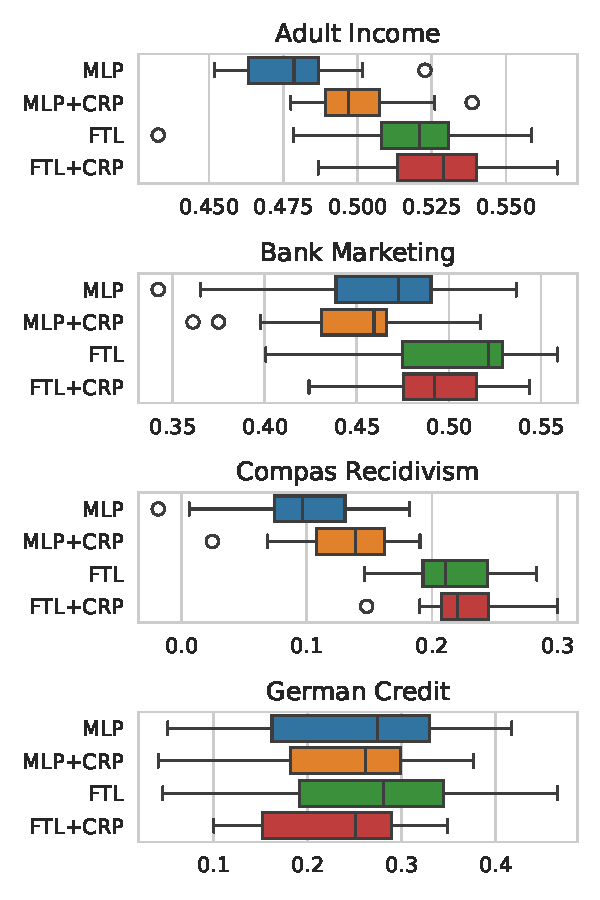
\includegraphics[width=1\linewidth]{images/boxplot_mcc_odds_crp.pdf}
\end{subfigure}
\end{figure}

\begin{figure}[!ht]
\centering
\caption{Fitness values of CRP optimizing Accuracy and multiple fairness metrics.}
\begin{subfigure}{.32\linewidth}
    \caption{Statistical Parity}
    \label{fig:boxplot_acc_parity_crp}
    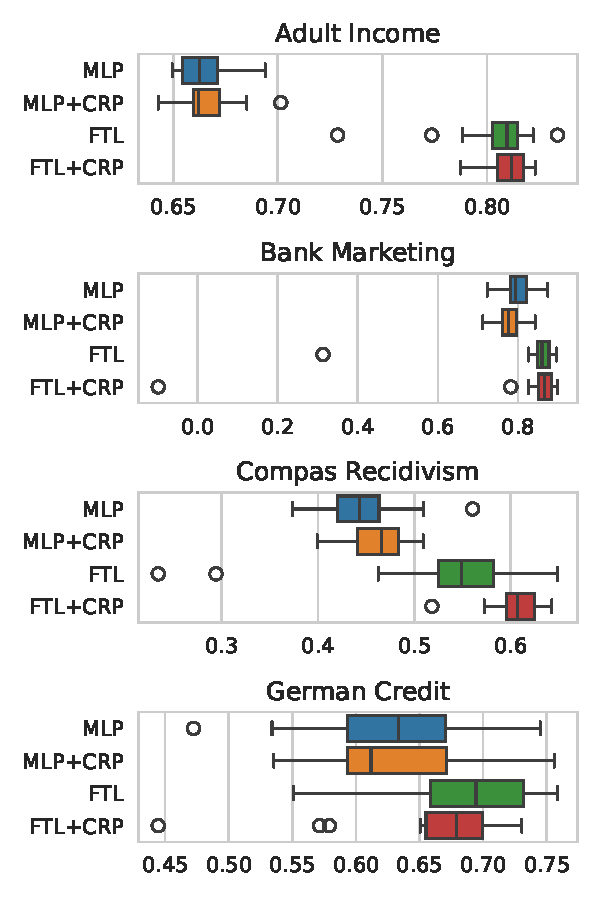
\includegraphics[width=1\linewidth]{images/boxplot_acc_parity_crp.pdf}
\end{subfigure}
\begin{subfigure}{.32\linewidth}
    \caption{Equal Opportunity}
    \label{fig:boxplot_acc_opp_crp}
    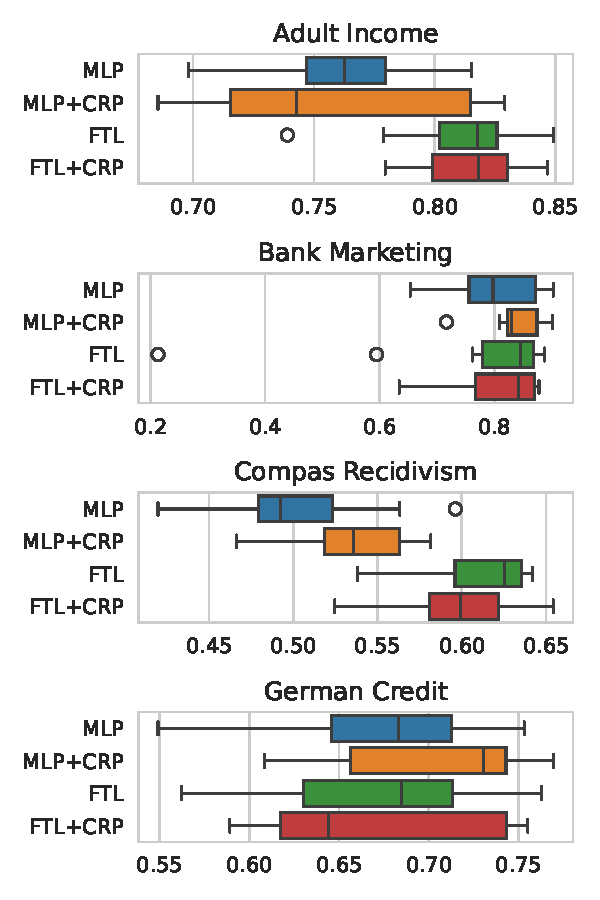
\includegraphics[width=1\linewidth]{images/boxplot_acc_opportunity_crp.pdf}
\end{subfigure}
\begin{subfigure}{.32\linewidth}
    \caption{Equalized Odds}
    \label{fig:boxplot_acc_odds_crp}
    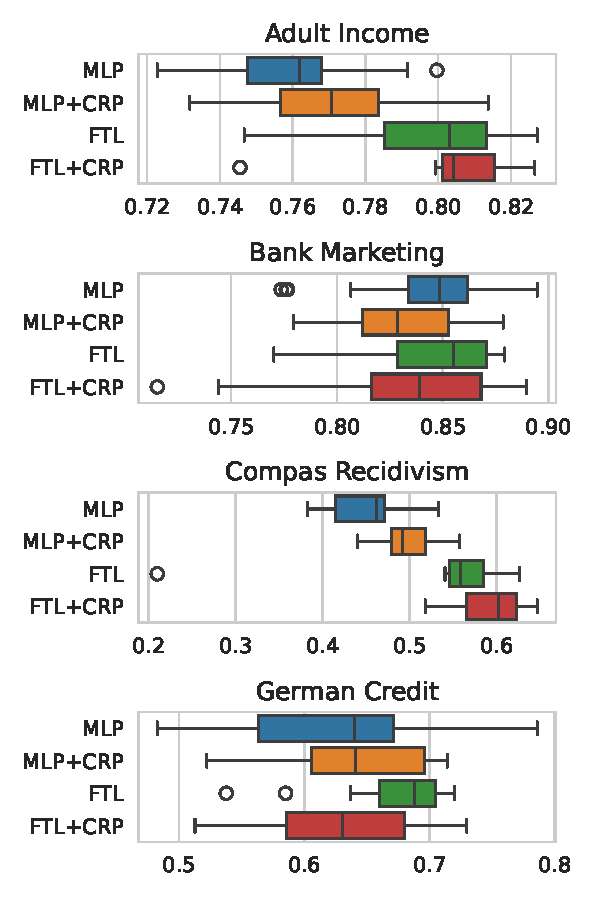
\includegraphics[width=1\linewidth]{images/boxplot_acc_odds_crp.pdf}
\end{subfigure}
\end{figure}



\begin{table}
    \centering
    \caption{Mean and standard deviation metric values optimizing MCC and Statistical Parity in comparison with Chatterjee Redlining Penalty.}\label{tab:complete_mcc_parity_crp}
    {\footnotesize\begin{tabular}{llrrr}
    \toprule
    Dataset & Method & Fitness & MCC & Stat. Parity \\
    \midrule

    \multirow[t]{4}{*}{Adult Income} & FTL+CRP & $0.494 (\pm0.01)$ & $0.517 (\pm0.02)$ & $0.023 (\pm0.02)$ \\
     & FTL & $0.487 (\pm0.02)$ & $0.509 (\pm0.02)$ & $0.022 (\pm0.02)$ \\
     & MLP+CRP & $0.388 (\pm0.01)$ & $0.578 (\pm0.01)$ & $0.191 (\pm0.01)$ \\
     & MLP & $0.386 (\pm0.01)$ & $0.576 (\pm0.01)$ & $0.191 (\pm0.01)$ \\
    \midrule
    \multirow[t]{4}{*}{Bank Marketing} & FTL & $0.534 (\pm0.03)$ & $0.569 (\pm0.01)$ & $0.035 (\pm0.03)$ \\
     & FTL+CRP & $0.523 (\pm0.04)$ & $0.569 (\pm0.01)$ & $0.046 (\pm0.04)$ \\
     & MLP & $0.429 (\pm0.03)$ & $0.521 (\pm0.02)$ & $0.092 (\pm0.02)$ \\
     & MLP+CRP & $0.426 (\pm0.05)$ & $0.528 (\pm0.02)$ & $0.102 (\pm0.04)$ \\
    \midrule
    \multirow[t]{4}{*}{Compas Recidivism} & FTL & $0.239 (\pm0.03)$ & $0.276 (\pm0.03)$ & $0.036 (\pm0.03)$ \\
     & FTL+CRP & $0.236 (\pm0.05)$ & $0.294 (\pm0.03)$ & $0.058 (\pm0.04)$ \\
     & MLP+CRP & $0.121 (\pm0.05)$ & $0.329 (\pm0.03)$ & $0.208 (\pm0.03)$ \\
     & MLP & $0.074 (\pm0.03)$ & $0.283 (\pm0.02)$ & $0.209 (\pm0.04)$ \\
    \midrule
    \multirow[t]{4}{*}{German Credit} & FTL+CRP & $0.302 (\pm0.06)$ & $0.371 (\pm0.05)$ & $0.069 (\pm0.05)$ \\
     & MLP & $0.266 (\pm0.10)$ & $0.329 (\pm0.09)$ & $0.064 (\pm0.05)$ \\
     & FTL & $0.256 (\pm0.12)$ & $0.355 (\pm0.08)$ & $0.099 (\pm0.06)$ \\
     & MLP+CRP & $0.246 (\pm0.07)$ & $0.329 (\pm0.05)$ & $0.084 (\pm0.06)$ \\
     \bottomrule
\end{tabular}}
\end{table}

 \begin{table}
    \centering
    \caption{Mean and standard deviation metric values optimizing MCC and Equal Opportunity in comparison with Chatterjee Redlining Penalty.}\label{tab:complete_mcc_opportunity_crp}
    {\footnotesize\begin{tabular}{llrrr}
    \toprule
    Dataset & Method & Fitness & MCC & Eq. Opp. \\
    \midrule

    \multirow[t]{4}{*}{Adult Income} & FTL+CRP & $0.554 (\pm0.03)$ & $0.581 (\pm0.02)$ & $0.027 (\pm0.02)$ \\
     & FTL & $0.540 (\pm0.04)$ & $0.576 (\pm0.01)$ & $0.036 (\pm0.03)$ \\
     & MLP+CRP & $0.506 (\pm0.05)$ & $0.577 (\pm0.01)$ & $0.071 (\pm0.05)$ \\
     & MLP & $0.480 (\pm0.04)$ & $0.582 (\pm0.01)$ & $0.103 (\pm0.04)$ \\
    \midrule
    \multirow[t]{4}{*}{Bank Marketing} & FTL & $0.483 (\pm0.07)$ & $0.567 (\pm0.02)$ & $0.084 (\pm0.06)$ \\
     & MLP & $0.420 (\pm0.08)$ & $0.524 (\pm0.02)$ & $0.104 (\pm0.08)$ \\
     & MLP+CRP & $0.420 (\pm0.10)$ & $0.529 (\pm0.02)$ & $0.109 (\pm0.09)$ \\
     & FTL+CRP & $0.416 (\pm0.14)$ & $0.519 (\pm0.15)$ & $0.104 (\pm0.08)$ \\
    \midrule
    \multirow[t]{4}{*}{Compas Recidivism} & FTL+CRP & $0.251 (\pm0.04)$ & $0.309 (\pm0.03)$ & $0.058 (\pm0.04)$ \\
     & MLP+CRP & $0.211 (\pm0.05)$ & $0.325 (\pm0.02)$ & $0.114 (\pm0.04)$ \\
     & FTL & $0.195 (\pm0.11)$ & $0.281 (\pm0.03)$ & $0.086 (\pm0.09)$ \\
     & MLP & $0.150 (\pm0.05)$ & $0.282 (\pm0.03)$ & $0.132 (\pm0.05)$ \\
    \midrule
    \multirow[t]{4}{*}{German Credit} & FTL & $0.293 (\pm0.12)$ & $0.368 (\pm0.10)$ & $0.074 (\pm0.05)$ \\
     & MLP & $0.290 (\pm0.09)$ & $0.355 (\pm0.07)$ & $0.065 (\pm0.06)$ \\
     & MLP+CRP & $0.275 (\pm0.09)$ & $0.341 (\pm0.06)$ & $0.066 (\pm0.05)$ \\
     & FTL+CRP & $0.166 (\pm0.16)$ & $0.284 (\pm0.14)$ & $0.117 (\pm0.07)$ \\
     \bottomrule
\end{tabular}}
\end{table}
 \begin{table}
    \centering
    \caption{Mean and standard deviation metric values optimizing MCC and Equalized Odds in comparison with Chatterjee Redlining Penalty.}\label{tab:complete_mcc_odds_crp}
    {\footnotesize\begin{tabular}{llrrr}
    \toprule
    Dataset & Method & Fitness & MCC & Eq. Odds \\
    \midrule

    \multirow[t]{4}{*}{Adult Income} & FTL+CRP & $0.526 (\pm0.02)$ & $0.575 (\pm0.01)$ & $0.048 (\pm0.02)$ \\
     & FTL & $0.515 (\pm0.03)$ & $0.572 (\pm0.02)$ & $0.057 (\pm0.02)$ \\
     & MLP+CRP & $0.500 (\pm0.02)$ & $0.578 (\pm0.01)$ & $0.078 (\pm0.02)$ \\
     & MLP & $0.478 (\pm0.02)$ & $0.575 (\pm0.01)$ & $0.097 (\pm0.02)$ \\
    \midrule
    \multirow[t]{4}{*}{Bank Marketing} & FTL & $0.495 (\pm0.05)$ & $0.574 (\pm0.01)$ & $0.078 (\pm0.05)$ \\
     & FTL+CRP & $0.490 (\pm0.03)$ & $0.571 (\pm0.01)$ & $0.081 (\pm0.03)$ \\
     & MLP & $0.461 (\pm0.05)$ & $0.522 (\pm0.02)$ & $0.061 (\pm0.04)$ \\
     & MLP+CRP & $0.446 (\pm0.04)$ & $0.539 (\pm0.02)$ & $0.093 (\pm0.04)$ \\
    \midrule
    \multirow[t]{4}{*}{Compas Recidivism} & FTL+CRP & $0.225 (\pm0.04)$ & $0.282 (\pm0.03)$ & $0.056 (\pm0.03)$ \\
     & FTL & $0.216 (\pm0.04)$ & $0.288 (\pm0.02)$ & $0.072 (\pm0.04)$ \\
     & MLP+CRP & $0.129 (\pm0.05)$ & $0.303 (\pm0.02)$ & $0.174 (\pm0.03)$ \\
     & MLP & $0.098 (\pm0.05)$ & $0.283 (\pm0.03)$ & $0.185 (\pm0.03)$ \\
    \midrule
    \multirow[t]{4}{*}{German Credit} & FTL & $0.278 (\pm0.12)$ & $0.383 (\pm0.08)$ & $0.105 (\pm0.06)$ \\
     & MLP & $0.249 (\pm0.10)$ & $0.352 (\pm0.08)$ & $0.102 (\pm0.06)$ \\
     & MLP+CRP & $0.231 (\pm0.10)$ & $0.332 (\pm0.07)$ & $0.102 (\pm0.06)$ \\
     & FTL+CRP & $0.228 (\pm0.08)$ & $0.337 (\pm0.07)$ & $0.109 (\pm0.06)$ \\
     \bottomrule
\end{tabular}}
\end{table}

 \begin{table}
    \centering
    \caption{Mean and standard deviation metric values optimizing Accuracy and Statistical Parity in comparison with Chatterjee Redlining Penalty.}\label{tab:complete_acc_parity_crp}
   {\footnotesize \begin{tabular}{llrrr}
    \toprule
    Dataset & Method & Fitness & Accuracy & Stat. Parity \\
    \midrule

    \multirow[t]{4}{*}{Adult Income} & FTL+CRP & $0.811 (\pm0.01)$ & $0.825 (\pm0.01)$ & $0.015 (\pm0.01)$ \\
     & FTL & $0.806 (\pm0.02)$ & $0.827 (\pm0.01)$ & $0.022 (\pm0.02)$ \\
     & MLP+CRP & $0.666 (\pm0.01)$ & $0.850 (\pm0.00)$ & $0.183 (\pm0.02)$ \\
     & MLP & $0.664 (\pm0.01)$ & $0.850 (\pm0.00)$ & $0.185 (\pm0.01)$ \\
    \midrule
    \multirow[t]{4}{*}{Bank Marketing} & FTL & $0.828 (\pm0.14)$ & $0.887 (\pm0.01)$ & $0.059 (\pm0.14)$ \\
     & FTL+CRP & $0.800 (\pm0.25)$ & $0.897 (\pm0.01)$ & $0.096 (\pm0.24)$ \\
     & MLP & $0.799 (\pm0.03)$ & $0.902 (\pm0.00)$ & $0.103 (\pm0.03)$ \\
     & MLP+CRP & $0.777 (\pm0.03)$ & $0.905 (\pm0.00)$ & $0.127 (\pm0.04)$ \\
    \midrule
    \multirow[t]{4}{*}{Compas Recidivism} & FTL+CRP & $0.606 (\pm0.03)$ & $0.651 (\pm0.01)$ & $0.045 (\pm0.03)$ \\
     & FTL & $0.520 (\pm0.12)$ & $0.619 (\pm0.04)$ & $0.100 (\pm0.11)$ \\
     & MLP+CRP & $0.462 (\pm0.03)$ & $0.659 (\pm0.01)$ & $0.197 (\pm0.03)$ \\
     & MLP & $0.439 (\pm0.04)$ & $0.646 (\pm0.01)$ & $0.207 (\pm0.04)$ \\
    \midrule
    \multirow[t]{4}{*}{German Credit} & FTL & $0.684 (\pm0.07)$ & $0.723 (\pm0.03)$ & $0.040 (\pm0.05)$ \\
     & FTL+CRP & $0.655 (\pm0.07)$ & $0.725 (\pm0.03)$ & $0.070 (\pm0.06)$ \\
     & MLP+CRP & $0.631 (\pm0.07)$ & $0.733 (\pm0.02)$ & $0.102 (\pm0.06)$ \\
     & MLP & $0.628 (\pm0.06)$ & $0.742 (\pm0.03)$ & $0.114 (\pm0.06)$ \\
     \bottomrule
\end{tabular}}
\end{table}


\begin{table}
    \centering
    \caption{Mean and standard deviation metric values optimizing Accuracy and Equal Opportunity in comparison with Chatterjee Redlining Penalty.}\label{tab:complete_acc_opportunity_crp}
    {\footnotesize \begin{tabular}{llrrr}
    \toprule
    Dataset & Method & Fitness & Accuracy & Eq. Opp. \\
    \midrule
    
    \multirow[t]{4}{*}{Adult Income} & FTL+CRP & $0.815 (\pm0.02)$ & $0.847 (\pm0.00)$ & $0.031 (\pm0.02)$ \\
     & FTL & $0.812 (\pm0.03)$ & $0.845 (\pm0.01)$ & $0.034 (\pm0.02)$ \\
     & MLP & $0.758 (\pm0.04)$ & $0.848 (\pm0.00)$ & $0.090 (\pm0.04)$ \\
     & MLP+CRP & $0.757 (\pm0.05)$ & $0.849 (\pm0.00)$ & $0.091 (\pm0.05)$ \\
    \midrule
    \multirow[t]{4}{*}{Bank Marketing} & MLP+CRP & $0.839 (\pm0.05)$ & $0.903 (\pm0.00)$ & $0.063 (\pm0.04)$ \\
     & MLP & $0.803 (\pm0.07)$ & $0.902 (\pm0.00)$ & $0.099 (\pm0.07)$ \\
     & FTL+CRP & $0.802 (\pm0.08)$ & $0.892 (\pm0.01)$ & $0.090 (\pm0.09)$ \\
     & FTL & $0.781 (\pm0.17)$ & $0.883 (\pm0.02)$ & $0.102 (\pm0.17)$ \\
    \midrule
    \multirow[t]{4}{*}{Compas Recidivism} & FTL & $0.614 (\pm0.03)$ & $0.645 (\pm0.03)$ & $0.031 (\pm0.02)$ \\
     & FTL+CRP & $0.598 (\pm0.03)$ & $0.639 (\pm0.02)$ & $0.041 (\pm0.03)$ \\
     & MLP+CRP & $0.536 (\pm0.03)$ & $0.663 (\pm0.01)$ & $0.127 (\pm0.03)$ \\
     & MLP & $0.498 (\pm0.04)$ & $0.646 (\pm0.01)$ & $0.148 (\pm0.04)$ \\
    \midrule
    \multirow[t]{4}{*}{German Credit} & MLP+CRP & $0.702 (\pm0.05)$ & $0.750 (\pm0.02)$ & $0.048 (\pm0.04)$ \\
     & FTL & $0.676 (\pm0.06)$ & $0.751 (\pm0.02)$ & $0.075 (\pm0.06)$ \\
     & MLP & $0.673 (\pm0.06)$ & $0.739 (\pm0.03)$ & $0.066 (\pm0.05)$ \\
     & FTL+CRP & $0.665 (\pm0.06)$ & $0.736 (\pm0.03)$ & $0.071 (\pm0.05)$ \\
     \bottomrule
\end{tabular} }
\end{table}

 \begin{table}
    \centering
    \caption{Mean and standard deviation metric values optimizing Accuracy and Equalized Odds in comparison with Chatterjee Redlining Penalty.}\label{tab:complete_acc_odds_crp}
    {\footnotesize \begin{tabular}{llrrr}
    \toprule
    Dataset & Method & Fitness & Accuracy & Eq. Odds \\
    \midrule
    
    \multirow[t]{4}{*}{Adult Income} & FTL+CRP & $0.805 (\pm0.02)$ & $0.843 (\pm0.01)$ & $0.038 (\pm0.02)$ \\
     & FTL & $0.798 (\pm0.02)$ & $0.841 (\pm0.01)$ & $0.043 (\pm0.02)$ \\
     & MLP+CRP & $0.772 (\pm0.02)$ & $0.849 (\pm0.00)$ & $0.077 (\pm0.02)$ \\
     & MLP & $0.760 (\pm0.02)$ & $0.849 (\pm0.00)$ & $0.089 (\pm0.02)$ \\
    \midrule
    \multirow[t]{4}{*}{Bank Marketing} & FTL & $0.846 (\pm0.03)$ & $0.890 (\pm0.01)$ & $0.044 (\pm0.04)$ \\
     & MLP & $0.845 (\pm0.03)$ & $0.901 (\pm0.00)$ & $0.057 (\pm0.03)$ \\
     & FTL+CRP & $0.831 (\pm0.05)$ & $0.892 (\pm0.01)$ & $0.061 (\pm0.05)$ \\
     & MLP+CRP & $0.830 (\pm0.03)$ & $0.902 (\pm0.00)$ & $0.072 (\pm0.03)$ \\
    \midrule
    \multirow[t]{4}{*}{Compas Recidivism} & FTL+CRP & $0.594 (\pm0.04)$ & $0.647 (\pm0.02)$ & $0.053 (\pm0.04)$ \\
     & FTL & $0.545 (\pm0.10)$ & $0.631 (\pm0.05)$ & $0.086 (\pm0.08)$ \\
     & MLP+CRP & $0.497 (\pm0.04)$ & $0.667 (\pm0.01)$ & $0.170 (\pm0.03)$ \\
     & MLP & $0.449 (\pm0.04)$ & $0.649 (\pm0.01)$ & $0.200 (\pm0.03)$ \\
    \midrule
    \multirow[t]{4}{*}{German Credit} & FTL & $0.669 (\pm0.05)$ & $0.712 (\pm0.02)$ & $0.043 (\pm0.07)$ \\
     & MLP+CRP & $0.640 (\pm0.06)$ & $0.748 (\pm0.02)$ & $0.107 (\pm0.06)$ \\
     & FTL+CRP & $0.631 (\pm0.06)$ & $0.721 (\pm0.03)$ & $0.090 (\pm0.08)$ \\
     & MLP & $0.619 (\pm0.07)$ & $0.740 (\pm0.03)$ & $0.121 (\pm0.07)$ \\
     \bottomrule
\end{tabular}}
\end{table}